\chapter{Seamless Shift of Focus} \label{chapter4}
\minitoc
\eject

The evolution of the economical constraints of a web application requires to continuously shift from productivity to efficiency.
The incompatibility between the two organizations implies technological ruptures during this evolution.
Huge developing efforts are pulled to translate manually from one organization into the other, and later to maintain the implementation despites its unmaintainable nature.

The proposition developed in this thesis is introduced in section \ref{chapter4:proposition}, and then developed throughout this chapter.

% It is based on the transformation of an event-driven program to target a pipeline architecture.
% The event-driven execution model on which relies the transformation is presented in section \ref{chapter4:event-driven}.
% Whereas the pipeline architecture targeted by the transformation, called the fluxional execution model, is presented section \ref{chapter4:flx-model}.
% Finally, the equivalence between the event-driven and the fluxional execution model is presented section \ref{chapter4:equivalence}.

% \begin{figure}[h!] \label{fig:state-of-the-art-proposition}
% \begin{center}
% 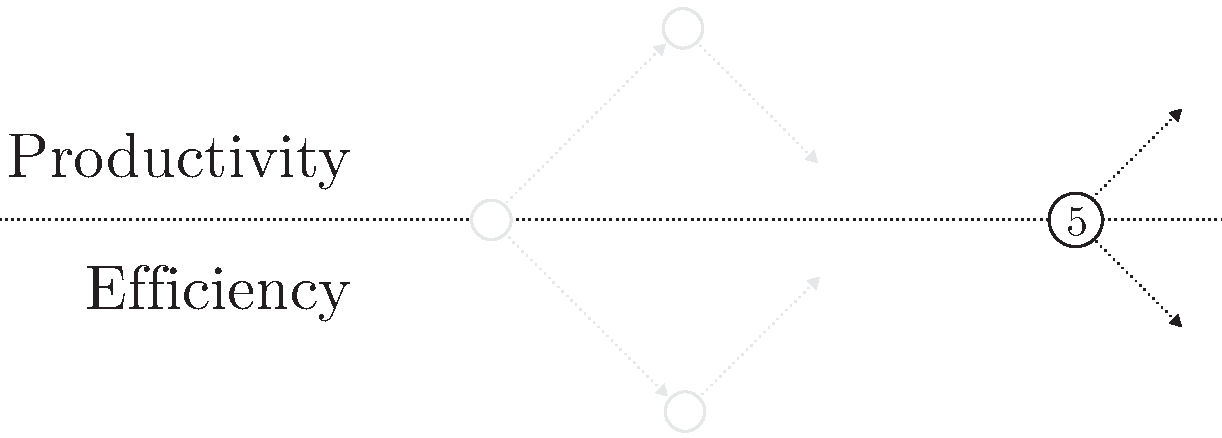
\includegraphics[width=0.6\textwidth]{../resources/state-of-the-art-5.pdf}
% \end{center}
% \end{figure}

\section{Proposition} \label{chapter2:proposition}

In the previous section, I presented two implementation organizations to improve either performance scalability, or development scalability.
However, these two organizations are incompatible, which imply ruptures in the development.
This thesis argues that a compiler should bridge the gap between the two organizations, so as to allow a continuous development.
This section presents the two programming models representing each an organization.
Then it presents the possibility of an equivalence between the two.
This equivalence is detailed further in the the chapter \ref{chapter4} and \ref{chapter5} of this thesis.

% I argue that the language should propose to the developer an abstraction to encourage the best practices of software development.
% Then a compiler, or the execution engine, can adapt this abstraction so as to leverage parallel architectures. 
% So as to provide to the developer a usable, yet efficient compromise.
% We propose to find an equivalence between the invariance proposed by the cooperative scheduling paradigm and the invariance proposed by the multi-processes paradigm in the case of web applications.

\subsection{Architecture of web applications}

\subsubsection{Real-time streaming web services}

% \nt{The need for invariance in the streaming applications : it can be emulated by message passing. Indeed the data flows from one processing step to the other, with few retroprogation of state (don't mention retro-propagation yet)}

We focus on web applications processing streams of requests from users in soft real-time.
Such applications receive requests from clients using the HTTP protocol and must respond within a finite window of time.
They are generally organized as sequences of tasks to modify the input stream of requests to produce the output stream of responses.
The stream of requests flows through the tasks, and is not stored.
% This stream of data stand out from the state of the application.
On the other hand, the state of the application remains in memory to impact the future behaviors of the application.
This state might be shared by several tasks within the application, and imply coordination between them.
% In this thesis I study two programming paradigm derived directly from the cooperative scheduling and the multi-process paradigms presented in previous sections to be applied in the case of real-time web applications.

The next paragraphs present two programming models to express web applications based on the invariance paradigms presented in the previous section.
%, the event-loop and the pipeline architecture.
The event-loop execution engine is based on the cooperative scheduling, and the pipeline architecture is based on isolated tasks communicating by message passing.
% They both feature different organization for the sequence of tasks, the stream and the state.
This thesis is based on the similarities between these two programming models.

\subsubsection{Event-loop}

The event-loop is an efficent execution model for concurrent applications on a single processing unit using non-blocking communications.
It relies on a queue storing the received messages before being processed one after the other by the loop.
On each reception, the loop executes a task to process the received message.
% This event is the aggregation of the response, and of a function to continue the execution with the result.
While processing the message, the task can initiate new communications, leading in turn to the queuing of more messages, which trigger more tasks, and so on.
The scheduling of execution is cooperative, each task is executed atomically and exclusively, until it yields execution, to continue with the next task in queue.


% The tasks are scheduled cooperatively, and yield execution on asynchronous communication.

In Javascript, these tasks are defined during the communication initiation.
The function called to initiate the execution expects as argument a function to continue the execution at the reception of communication result.
This function is called a callback or a continuation.

In this model, the input stream of data flows through a sequence of callbacks to be processed until the application outputs it.
This stream is never stored, except as a buffer between two callbacks.
On the contrary, The state ramins in memory to be shared by all callbacks.
Because Javascript is of higher-order, the callbacks as well as their execution contexts are part of this state.
They are called closures.
% In Javascript, it includes the closures.

\nt{TODO schema of an event-loop}

This execution model is similar to the pipeline architecture presented in the next paragraph.

\subsubsection{Pipeline}

The pipeline software architecture is composed of isolated stages communicating by message passing to leverage the parallelism of a multi-core hardware architectures.
It is well suited for streaming application, as the stream of data flows from stage to stage.
Each stage has an independent memory to hold its own state.
As the stages are indendent, the state coordination between the stages are communicated along with the stream of data.

\nt{TODO schema of a pipeline}

Each stage is organized in a similar fashion than the event-loop presented above.
It receives and queues messages from upstream stages, processes them one after the other, and outputs the result to downstream stages.
The difference is that in the pipeline architecture, each task is executed on an isolated stage, whereas in the event-loop execution model, all tasks share the same queue, loop and memory store.

Both paradigms encapsulate the execution in tasks assured to have an exclusive access to the memory.
However, they provide two different models to provide this exclusivity resulting in two distinct ways for the developer to assure the invariance on the application state.
Contrary to the pipeline architecture, the event-loop provide a common memory store allowing the best practice of software development to improve maintainability.
It is possibly the reason of the wide adoption of this programming model by the community of developers.

\paragraph{}

This thesis proposes to provide an equivalence between the two memory models for streaming web applications.
The next subsection describes further the similarities and differences between the two models.
The equivalence would allow a compiler to transform an application expressed in one model into the other.
With such a tool, a development team could rely on the common memory store of the event-loop execution model, and focus on the maintainability of the implementation.
And compile continuously during the development the event-loop implementation to the pipeline architecture to assure that the execution can be distributed on a parallel architecture.

\subsection{Equivalence}

\subsubsection{Rupture point}

The execution of the pipeline architecture is well delimited in isolated stages.
Each stage has its own thread of execution, and is independent from the others.
On the contrary, the code of the event-loop is linear because of the continuation passing style and the common memory store.
% The message passing linking the callbacks is transparently handled by the event-loop.
However, the execution of the different callbacks are as distinct as the execution of the different stages of a pipeline.
The call stacks of two callbacks are distincts.
Therefore, an asynchronous function call represents the rupture between two call stacks.
It is a rupture point, and is equivalent to a data stream between two stages in the pipeline architecture.

Both the pipeline architecture and the event-loop present these rupture points.
The detection of rupture points allows to map a pipeline architecture onto the implementation following the event-loop model.
To allow the transformation from one to the other, this thesis studies the possibility to detect rupture points, and to distribute the global memory into the parts defined by these rupture points.
The detection of rupture points is addressed in chapter \ref{chapter4}.

\subsubsection{Invariance}

% This transformation is important on two points.
% The conservation of the invariance.
% The equivalence between the coordinations.

The transformation should preserve the invariance as expressed by the developer to assure the correctness of the execution.
The partial ordering of events in a system, by opposition to total ordering, is sufficient to assure this correctness.
% This result was used by Lamport to prove the correctness of distributed systems.
The global memory is a way to assure the total ordering of events, and the message passing coordination is a way to assure partial ordering of events.
Therefore, to assure the correctness of the execution of a system, the state coordination with a global memory is equivalent to message passing coordination.
And it is possible, at least for some rupture points, to transform the global memory coordination into message passing while conserving the correctness of execution.

In order to preserve the invariance assured by the event-loop model after the transformation, each stage of the pipeline needs to have an exclusive access to memory.
The global memory needs not to be splited into parts and distributed into each of the stages.
To assure the missing coordinations assured by the shared memory between the stages, the transformation should provide equivalent coordination with message passing.
The isolation and replacement of the global memory is fully address in chapter \ref{chapter5}

% The invariance holds for the whole memory during the execution of each callback.
% As I explained in the previous section, this invariance is required to allow the concurrent execution of the different tasks.
% On the other hand, the invariance is explicit in the pipeline architecture, as all the stages have isolated memories.
% The coordination between these isolated process is made explicit by the developer through message passing.

% I argue that the state coordination between the callbacks requireing a global memory could be replaced by the message passing coordination used manually in the pipeline architecture.
% I argue that not all applications need concurrent access on the state, and therefore, need a shared memory.
% % Specifically, I argue that each state region remains roughly local to a stage during its modification.
% \nt{TODO review that, I don't know how to formulate these paragraphs. Identify the state and the data in the global memory.}

% \subsubsection{Transformation}

% This equivalence should allow the transformation of an event loop into several parallel processes communicating by messages.
% In this thesis, I study the static transformation of a program, but the equivalence should also hold for a dynamic transformation.
% I present the analyzis tools I developed to identify the state and the data from the global memory.

With this compiler, it would be possible to express an application following the design principles of software development, hence maintainable.
And yet, the execution engine could adapt itself to any parallelism of the computing machine, from a single core, to a distributed cluster.
Because of the equivalence between these two models, the development team could iterate testing the two models for their different concerns about the implementation : performance and maintainability.

The goal of conciling these two concerns is not new.
The next chapter presents all the results from previous works needed to understand this work, up to the latest results in the field.

\endinput




---


There are different kinds of state dependencies in applications components leading to different kinds of parallelism.
In this thesis I argue that it is possible to parallelize a real-time web applications written on an event-loop because the strong dependencies mainly remains within a closed number of concurrent executions.




\subsubsection{Learning curve}

Because the compiler intend to warn the developer about shared states, it would be a great tool for beginner to progressively adapt to the flow programming model and best practices.


\subsection{Liquid IT}

The goal of Liquid IT is to hide the technical complexity of scalability to the developer, so he can focus solely on business logic.



\section{Execution Models} \label{chapter4:execution-models}

The event-driven execution model and the pipeline execution model were already briefly presented in chapter \ref{chapter2}, section \ref{chapter2:web-as-a-platform:web-servers}, page \pageref{chapter2:web-as-a-platform:web-servers}.
The next paragraphs dive into the details of each execution model in regard of the transformation.

\subsection{Event-Driven Execution Model} \label{chapter4:event-driven}

The event-driven execution model processes a queue of asynchronous events by cooperatively scheduling handlers.
To respond to an event, the associated handler can directly respond to the source of the event.
Or it can request an external resource, and chain another handler to later process the initial event with the resource response, as illustred in figure \ref{fig:cont-chain}.
The developer defines each handler as a continuation and defines their causality using the continuation passing style \cite{Wand1980,Haynes1984}.

\begin{figure}[h!]
  \centering
  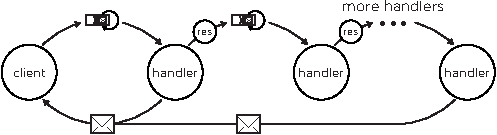
\includegraphics[width=0.7\linewidth]{../resources/cont-chain.pdf}
  \caption{Chain of continuations}
  \label{fig:cont-chain}
\end{figure}

\subsubsection{Continuation Passing Style} \label{chapter4:event-loop:continuation}

% A callback is a function passed as a parameter to a function call.
% It is invoked by the callee to continue the execution with data not available in the caller context.
% We distinguish three kinds of callbacks.

% \begin{description}
%   \item[Iterators] are functions called for each item in a set, often synchronously.
%   \item[Listeners] are functions called asynchronously for each event in a stream.
%   \item[Continuations] are functions called asynchronously once a result is available.
% \end{description}

% In a synchronous paradigm, the sequentiality of the execution flow is trivial.
% An operation needs to complete before executing the next one.
% In an asynchronous paradigm, parallelism is trivial, but the sequentiality of operations needs to be explicit.

% A continuation is the functional way of defining the causality between two tasks \cite{Wand1980,Haynes1984}.
A continuation is a function passed as an argument to a function call.
% The caller is able to continue the execution while the callee runs in background.
The continuation is invoked after the completion of the callee, to continue the execution. % as soon as possible and process the result; hence the name continuation.
In the event-driven execution model, the continuation is invoked as a new handler, to avoid blocking the caller until its completion.
% It provides a necessary control over the asynchronous execution flow.
% It also brings a control over the data flow which essentially replaces the \texttt{return} statement at the end of a synchronous function.
At its invocation, the continuation retrieves both the caller context and the result of the callee through a closure.
Listing \ref{lst:continuation} illustrates an example of continuation in \textit{Node.js}.

% The convention on how to hand back the result must be common for both the callee and the continuation.
% For example, in \textit{Node.js}, the signature of a continuation uses the \textit{error-first} convention.
% % \ftnt{https://docs.nodejitsu.com/articles/errors/what-are-the-error-conventions}
% % \ftnt{http://programmers.stackexchange.com/questions/144089/different-callbacks-for-error-or-error-as-first-argument} convention.
% The first argument contains an error or \texttt{null} if no error occurred; then follows the result.
% Listing \ref{lst:continuation} is a pattern of such a continuation.
% However, continuations don't impose any conventions; indeed, other conventions are used in the browser.

\begin{code}[js, %
             caption={Example of a continuation}, %
             label={lst:continuation}] %
callee(input, function continuation(error, result) {
  if (error)
    throw error;
  // ... modify result
  console.log(result);
});
\end{code}

% % The continuation allows to continue the execution sequentially, after the result of \textit{my_fn} is available.
% % When continuations are defined inside the call, like \textit{continuation}, the sequence of deferred execution results in an intricate imbrication of calls and continuations, like in listing \ref{lst:cbhell}.
% The callback hell occurs when many asynchronous calls are arranged to be executed sequentially.
% Each consecutive operation adds an indentation level, because it is nested inside the continuation of the previous operation.
% % That is when each caller must wait for the result before calling the next function.
% It produces an imbrication of calls and function definitions, as shown in listing \ref{lst:cbhell}.

Asynchronous continuations cannot be composed to chain their execution like synchronous functions, as illustrated in listing \ref{lst:cbhell}.
This nested construction is sometime difficult to follow.
% The continuation passing style lacks the chained composition of multiple asynchronous operations.
% It forces to stack calls of continuations, as illustrated in listing \ref{lst:cbhell}.
Promises improve continuations to allow this composition.
They allow to arrange a sequence of asynchronous operations in a chain, similar to a pipeline.

\begin{code}[js, %
             caption={Example of a sequence of continuations}, %
             label={lst:cbhell}] %

callee(input, function continuation(error, result) {
  if (error)
    throw error;
  // ... modify result
  nestedCallee(result, function continuation(error, nestedResult) {
    if (error)
      throw error;
    // ... modify result
    superNestedCallee(nestedResult, function continuation(error, superNestedResult) {
      // ... and so on ...
    }
  });
});
\end{code}

\subsubsection{Promise} \label{chapter4:event-loop:promise}

% TODO insert these :
% Promise also provide few methods to enhance the asynchronous control flow tools\footnote{\texttt{all} and \texttt{race}}.
% There is, in Javascript, numerous Promise implementations\footnote{37 different implementations in Javascript \url{https://github.com/promises-aplus/promises-spec/blob/master/implementations.md}}.

% This section is based on the Promises section of the specification in ECMAScript 6 Harmony\ftnt{https://people.mozilla.org/~jorendorff/es6-draft.html\#sec-promise-objects} and the Promises page on the Mozilla Developer Network\ftnt{https://developer.mozilla.org/en/docs/Web/JavaScript/Reference/Global_Objects/Promise}.

% In a synchronous paradigm, the sequentiality of the execution flow is trivial.
% In the asynchronous paradigm, the control over the asynchronous execution flow is defined with continuations.
% In the asynchronous paradigm, this control is provided by continuations.
% Promises provide a unified control over the execution flow for both paradigms.
% The ECMAScript 6 specification\ftnt{https://people.mozilla.org/~jorendorff/es6-draft.html\#sec-promise-objects} defines
A Promise is used as a placeholder for the eventual outcome of a deferred (and possibly asynchronous) operation.
Listing~\ref{lst:then} illustrates a simple promise.
% A Promise is an object returned by a function to represent its result
In Javascript, promises expose a \texttt{then} method which expects a continuation to continue the execution with the result of the deferred operation. %; this result being synchronously or asynchronously available.
This method allows to chain Promises one after the other, as illustrated in listing~\ref{lst:promises-sequence}.

% However, unlike continuations, the Promises specification imposes a convention on how to handle the result.
% Because it is possibly unavailable synchronously, it still requires a continuation to defer the execution when the result is made available.
% A promise requires two continuations to defer the execution in case of errors.
% These two continuations are passed to the \texttt{then} method of the promise, like illustrated in listing \ref{lst:then}.

% As a result of this difference, Promises and continuations use two different conventions to handle errors and results.
% The two conventions are illustrated in listings \ref{lst:continuation} and \ref{lst:then}.

\begin{code}[js, %
             caption={Example of a Promise}, %
             label={lst:then}] %
var promise = callee(input)

promise.then(function onSuccess(result) {
  console.log(result);
}, function onError(error) {
  throw error;
});
\end{code}

% Continuations lack the chained composition of asynchronous operations.
% Promises are designed to fill the lack of chained composition from continuations.
% They allow to arrange successions of asynchronous operations as a chain of continuations, by opposition to the imbrication of continuations illustrated in listing \ref{lst:cbhell}.
% That is to arrange them, one operation after the other, in the same indentation level.
% The \texttt{then} method synchronously returns a Promise linked with the Promise asynchronously returned by its continuation.
% This link allow to compose chains of asynchronous operations.


% The functions \texttt{callee\_promise\_2} and \texttt{callee\_promise\_3} return promises when they are executed.
% They are executed asynchronously, so these promises are not available synchronously.
% The method \texttt{then} synchronously returns intermediary Promises to bridge with the asynchronous promises.
% The former resolves when the latter resolves.
% The latter resolve only when the former resolve.
% This behavior allows to arrange the continuations as a flat chain of calls, instead of an imbrication of continuations.

\begin{code}[js, %
             caption={Example of a chain of Promises}, %
             label={lst:promises-sequence}] %
callee_promise_1(input)
.then(callee_promise_2, onError)
.then(callee_promise_3, onError)
.then(console.log, onError);

function onError(error) {
  throw error;
}
\end{code}

% The Promises syntax is more concise, and also more readable because it is closer to the familiar synchronous paradigm.
% Indeed, Promises allow to arrange both the synchronous and asynchronous execution flow with the same syntax.
Promises allow to easily arrange the execution flow in parallel or in sequence according to the required causality.
% This control over the execution leads to a modification of the control over the data flow.
Programmers are encouraged to arrange the computation as series of steps to process incoming events and yield outcoming events.
In this sense, Promises are an intermediate step toward the pipeline execution model.



\subsection{Fluxional Execution Model} \label{chapter4:flx-model}

The fluxional execution model is inspired by the pipeline architecture.
It is the target for the transformation presented in this thesis.
It executes programs written in the fluxional language, whose grammar is presented in figure \ref{fig:flx-lang}.
It intends to provide scalability to web applications with a granularity of parallelism at the function level.

The functions of an application $\bnfpn{program}$ are encapsulated in autonomous execution containers named \textit{fluxions} $\bnfpn{flx}$.

\begin{figure}[h]
\vspace{-0.6\baselineskip}
\begin{bnf*}
  \bnfprod{program}    {\bnfpn{flx} \bnfor \bnfpn{flx} \bnfsp \bnftd{eol} \bnfsp \bnfpn{program}}\\
  \bnfprod{flx}        {\bnfts{\texttt{flx}} \bnfsp \bnfpn{id} \bnfsp \bnfpn{tags} \bnfsp \bnfpn{ctx} \bnfsp \bnftd{eol} \bnfsp \bnfpn{streams} \bnfsp \bnftd{eol} \bnfsp \bnfpn{fn}}\\
  \bnfprod{tags}       {\bnfts{\texttt{\&}} \bnfsp \bnfpn{list} \bnfor \bnftd{empty string}}\\
  \bnfprod{streams}    {\bnfts{\texttt{null}} \bnfor \bnfpn{stream} \bnfor \bnfpn{stream} \bnfsp \bnftd{eol} \bnfsp \bnfpn{streams}}\\
  \bnfprod{stream}     {\bnfpn{type} \bnfsp \bnfpn{dest} \bnfsp [\bnfpn{msg}]}\\
  \bnfprod{dest}       {\bnfpn{list}}\\
  \bnfprod{ctx}        {\bnfts{\texttt{\{}} \bnfpn{list} \bnfts{\texttt{\}}}}\\
  \bnfprod{msg}        {\bnfts{\texttt{[}} \bnfpn{list} \bnfts{\texttt{]}}}\\
  \bnfprod{list}       {\bnfpn{id} \bnfor \bnfpn{id} \bnfsp \bnfts{,} \bnfsp \bnfpn{list}}\\
  \bnfprod{type}       {\bnfts{\texttt{>}\texttt{>}} \bnfor \bnfts{\texttt{-}\texttt{>}}}\\
  \bnfprod{id}         {\bnftd{Identifier}}\\
  \bnfprod{fn}         {\bnftd{Source language with~} \bnfpn{stream} \bnftd{~placeholders}}\\
\end{bnf*}
\vspace{-2.5\baselineskip}
\caption{Syntax of a high-level language to represent a program in the fluxional form}
\label{fig:flx-lang}
\end{figure}


% The following paragraphs present the \textit{fluxions} and the messaging system to carry the communications between \textit{fluxions}.
% , and then an example application using this execution model.

% \subsubsection{Fluxions and Messaging System}

\subsubsection{Fluxion}

A \textit{fluxion} $\bnfpn{flx}$ is named by a unique identifier $\bnfpn{id}$ to receive messages, and might be part of one or more groups indicated by tags $\bnfpn{tags}$.
A \textit{fluxion} is composed of a processing function $\bnfpn{fn}$, and a local memory called a \textit{context} $\bnfpn{ctx}$.

At a message reception, the \textit{fluxion} modifies its \textit{context}, and sends messages to downstream \textit{fluxions} on its output streams $\bnfpn{streams}$.
The \textit{context} stores the state on which a \textit{fluxion} relies between two message receptions, similarly to the actors model.
The messaging system queues the output messages for the event loop to process them later by calling the downstream \textit{fluxions}.

% And the communications are similar to the dataflow programming model, which allows to reason on the throughput of these streams, and to react to load increases \cite{Bartenstein2014}.

In addition to message passing, the execution model allows \textit{fluxions} to communicate by sharing state between their \textit{contexts}.
The fluxions that need this synchronization are grouped with the same tag, and loose their independence.

\subsubsection{Streams}

There are two types of streams, \textit{start} and \textit{post}, which correspond to the nature of the rupture point producing the stream.
A \textit{start} rupture point starts a chain of continuations, while a \textit{post} rupture point is a continuation in a chain.
\textit{Start} streams are indicated with a double arrow ($\to$ \hspace{-1.4em} $\to$ or \texttt{>>}) and \textit{post} streams with a simple arrow ($\to$ or \texttt{->}).

The variables defined before the \textit{start} are available for the whole chain, and require synchronization for concurrent execution of the same chain.
Whereas the variables defined inside the chain are available only in this chain, and don't require synchronization.
% A variable created within a chain of \textit{post} streams requires more synchronization than a variable created upstream a \textit{start} stream.
The two types and implications of rupture points are further detailed in section \ref{chapter5:flx:compiler}.

\subsection{Example}

\begin{code}[js,
  caption={Example web application},
  label={lst:source}]
var app = require('express')(),
    fs = require('fs'),
    count = 0; //@\label{lst:source-counter}@

app.get('/', function handler(req, res){ //@\label{lst:source-handler}@
  fs.readFile(__filename, function reply(err, data) {
    count += 1;
    res.send(err || template(count, data)); //@\label{lst:source-send}@
  });
}); //@\label{lst:source-handler-end}@

app.listen(8080);
\end{code}

\begin{figure}[h!]
  \centering
  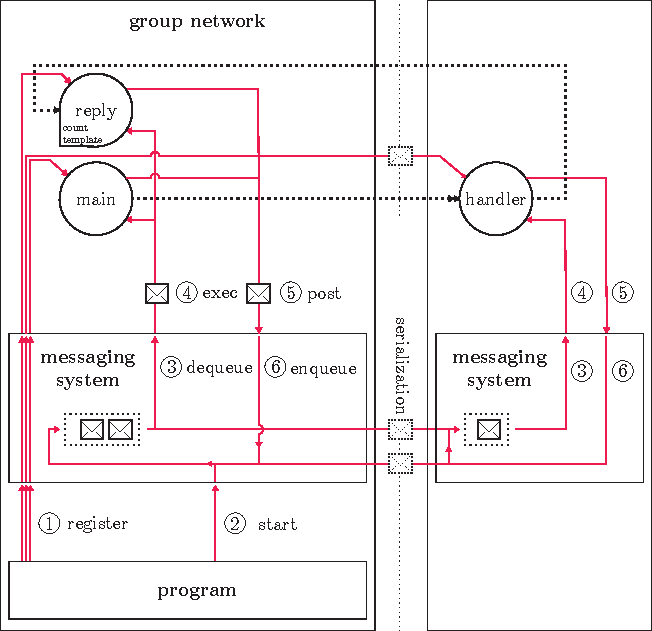
\includegraphics[width=0.7\linewidth]{../resources/schema-message.pdf}
  \caption{The fluxional execution model in details}
  \label{fig:MesSys}
\end{figure}

% \begin{wrapfigure}{r}{0.60\textwidth}
%   \vspace{-25pt}
%   \begin{center}
%     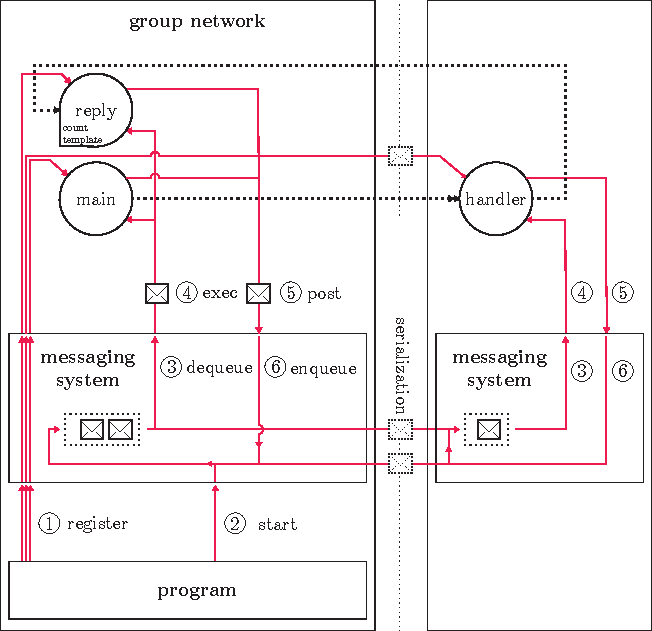
\includegraphics[width=\linewidth]{../resources/schema-message.pdf}
%     \caption{The fluxional execution model in details}
%     \label{fig:MesSys}
%   \end{center}
%   \vspace{-10pt}
% \end{wrapfigure}

% The fluxional execution model is illustrated with an example application presented in listing \ref{lst:source}.
The example application in listing \ref{lst:source} reads a file, and sends it back along with a request counter.
The \texttt{handler} function, line \ref{lst:source-handler} to \ref{lst:source-handler-end}, receives the input stream of requests.
The \texttt{count} variable at line \ref{lst:source-counter} counts the requests, and needs to be saved between two messages receptions.
The \texttt{template} function formats the output stream to be sent back to the client.
The \texttt{app.get} and \texttt{res.send} functions, lines \ref{lst:source-handler} and \ref{lst:source-send}, interface the application with the clients.
Between these two interface functions is a chain of three functions to process the client requests : \texttt{app.get} $\to$ \hspace{-1.4em} $\to$ \texttt{handler} $\to$ \texttt{reply}.
This chain of functions is transformed into a pipeline, expressed in the high-level fluxional language in listing \ref{lst:fluxional}.
The transformation process between the source and the fluxional code is explained in \ref{chapter5}, in section \ref{chapter5:flx:compiler}.

The execution is illustrated in figure \ref{fig:MesSys}.
The dashed arrows between fluxions represent the message streams as seen in the fluxional application.
The plain arrows represent the operations of the messaging system during the execution.
These steps are indicated by numeroted circles.
The \textit{program} registers its fluxions in the messageing system, \circled{1}.
The fluxion \textit{reply} has a context containing the variable \texttt{count} and \texttt{tem\-plate}.
When the application receives a request, the first fluxion in the stream, \textit{main}, queues a \texttt{start} message containing the request, \circled{2}.
This first message is to be received by the next fluxion \textit{handler}, \circled{3}, and triggers its execution, \circled{4}.
The fluxion \textit{handler} sends back a message, \circled{5}, to be enqueued, \circled{6}.
The system loops through steps \circled{3} through \circled{6} until the queue is empty.
This cycle starts again for each new incoming request causing another \texttt{start} message.

\begin{code}[flx, caption={Example application expressed in the high-level fluxional language}, label={lst:fluxional}]
flx main & grp_res
>> handler [res]
  var app = require('express')(),
      fs = require('fs'),
      count = 0;

  app.get('/', >> handler); //@\label{lst:fluxional-streamtohandler}@
  app.listen(8080);

flx handler
-> reply [res]
  function handler(req, res) {
    fs.readFile(__filename, -> reply); //@\label{lst:fluxional-readfile}@
  }

flx reply & grp_res {count, template}
-> null
  function reply(error, data) {
    count += 1; //@\label{lst:fluxional-counter}@
    res.send(err || template(count, data)); //@\label{lst:fluxional-ressend}@
  }
\end{code}

The chain of functions from listing \ref{lst:source} is expressed in the fluxional language in listing \ref{lst:fluxional}.
The fluxion \texttt{handler} doesn't have any dependencies, so it can be executed in a parallel event-loop.
The fluxions \texttt{main} and \texttt{reply} belong to the group \texttt{grp\_res}, indicating their dependency over the variable \texttt{res}.
The group name is chosen arbitrarily.
All the fluxions inside a group are executed sequentially on the same event-loop, to protect the shared variables against concurrent accesses.

The variable \texttt{res} is created and consumed within a chain of \textit{post} stream.
Therefore, it is exclusive to one request and cannot be propagated to another request.
It doesn't prevent the whole group from being replicated.
However, the fluxion \texttt{reply} depends on the variable \texttt{count} created upstream the \textit{start} stream, which prevents this replication.
If it did not rely on this state, the group \texttt{grp\_res} would be stateless, and could be replicated to cope with the incoming traffic.

\separator

This execution model allows to parallelize the execution of an application as a pipeline, as with the fluxion \texttt{handler}.
And some parts are replicated, as could be the group \texttt{grp\_res}.
This parallelization improves the efficiency of the application.
Indeed, as a fluxion contains its state and expresses its dependencies, it can be migrated.
It allows to adapt the number of fluxions per core to adjust the resource usage in function of the desired throughput.

Yet, the parallelization is limited by the dependencies between fluxions.
A developer can ignore these dependencies at first, to focus on productivity.
And then continuously tune the implementation to remove these dependencies and improve efficiency.
This continuous tuning avoid the disruptive shifts of technology required by current platforms.
% \section{Equivalence} \label{chapter4:equivalence}

The goal of this thesis is not to propose a new high-level language but to automate the architectural shift.
The next paragraphs introduces the equivalence between the memory abstraction of the event-driven execution model and of the pipeline architecture previously presented.
The equivalence is broken down in two steps, as illustrated in figure \ref{fig:chapter4:roadmap}.
The first step identifies the stages of the pipeline and the rupture points between them in the control flow.
The second step enforces isolation of memory between these stages to preserve invariance.

\begin{figure}[h!]
\begin{center}
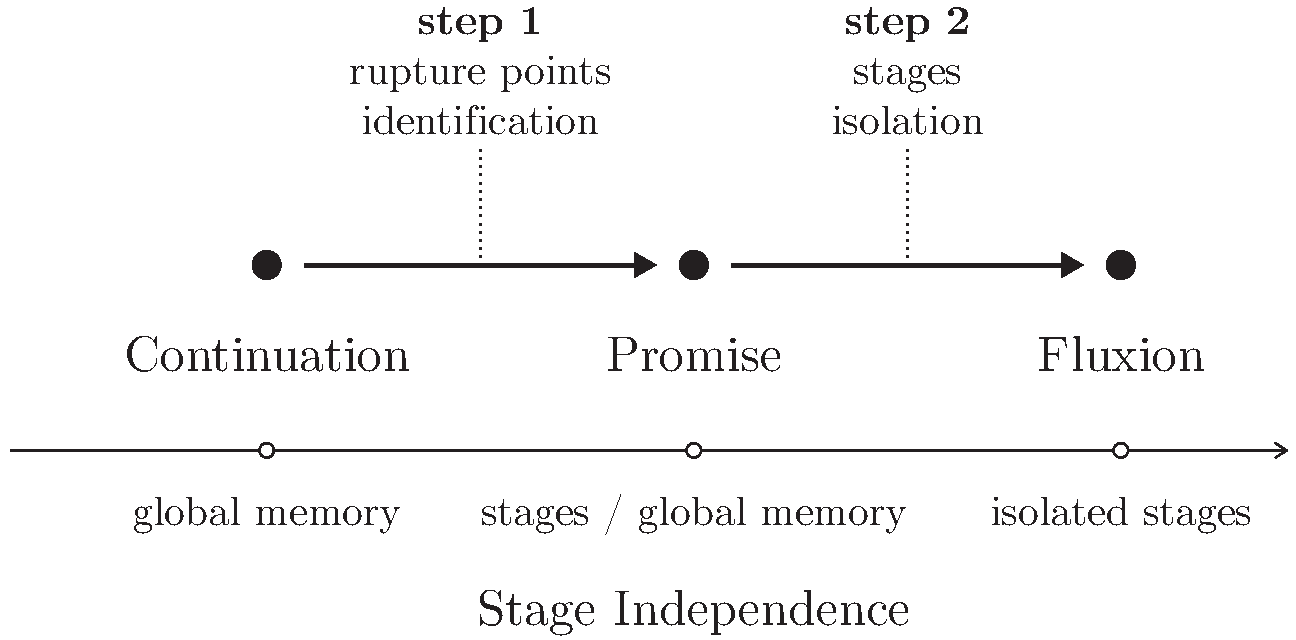
\includegraphics[width=0.9\textwidth]{../resources/roadmap.pdf}
\end{center}
\caption{Roadmap}
\label{fig:roadmap}
\end{figure}

\subsection{Rupture Point}

The pipeline architecture enforces the memory isolation between stages.
Each stage has its own thread of execution, and is independent from the others.
On the other hand, the execution flow of the event-loop jumps from one concurrent task to the other.
%  because of the continuation passing style and the common memory store.
% The message passing linking the callbacks is transparently handled by the event-loop.
However, the executions of these tasks are as distinct as the execution of the different stages of a pipeline.
The call stacks of two concurrent tasks are distinct.
The asynchronous function call between the caller and its continuation represents the rupture between two call stacks.
It is a rupture point, and is equivalent to a data stream between two stages in the pipeline architecture.

Both the pipeline architecture and the event-loop present these rupture points.
The detection of rupture points allows to map a pipeline architecture onto the implementation following the event-loop model.
To allow the transformation from one to the other, this thesis studies the possibility to detect rupture points, and to distribute the global memory into the parts defined by these rupture points.

The detection of rupture points is addressed in chapter \ref{chapter5}.
It presents the extraction of a pipeline of concurent tasks from a Javascript application.
Such pipeline is similar to the one exposed by Promises.
% The chapter proposes a simpler alternative to the latter called Dues.
However, these concurent tasks still require a global memory.
They can't be executed in parallel.

\subsection{Invariance}

% This transformation is important on two points.
% The conservation of the invariance.
% The equivalence between the coordinations.

The global memory assures the total ordering of tasks, and requires sequentiality, while message passing assures causal ordering of tasks and allows parallelism.
The causal ordering of tasks, by opposition to total ordering, is sufficient to assure the correctness of the execution.
Therefore, to assure the correctness of the execution, the ordering allowd by the global memory is partially equivalent to message passing ordering.
And it is possible to transform the global memory coordination into message passing.
% Given that the tasks are independent and communicate by messages.

% This result was used by Lamport to prove the correctness of distributed systems.
Yet, to preserve the correctness as expressed by the developer, it is important to preserve the invariance.
The global memory needs not to be distributed into each of the stages of the pipeline, so that each stage have an exclusive access to its memory.

To assure the missing coordinations assured by the shared memory between the stages, the transformation should provide equivalent coordination with message passing.
The isolation and replacement of the global memory is addressed in chapter \ref{chapter6}, with the introduction of isolated containers called Fluxions.




% The invariance holds for the whole memory during the execution of each callback.
% As I explained in the previous section, this invariance is required to allow the concurrent execution of the different tasks.
% On the other hand, the invariance is explicit in the pipeline architecture, as all the stages have isolated memories.
% The coordination between these isolated process is made explicit by the developer through message passing.

% I argue that the state coordination between the callbacks requireing a global memory could be replaced by the message passing coordination used manually in the pipeline architecture.
% I argue that not all applications need concurrent access on the state, and therefore, need a shared memory.
% % Specifically, I argue that each state region remains roughly local to a stage during its modification.
% \nt{TODO review that, I don't know how to formulate these paragraphs. Identify the state and the data in the global memory.}

% \subsubsection{Transformation}

% This equivalence should allow the transformation of an event loop into several parallel processes communicating by messages.
% In this thesis, I study the static transformation of a program, but the equivalence should also hold for a dynamic transformation.
% I present the analyzis tools I developed to identify the state and the data from the global memory.